\subsection{S1. Data and processing
details}\label{s1.-data-and-processing-details}

The implementation is not an object of the theoretical guarantees, so
the processing is fixed in code and the choices that determine the
output are listed here in full.

\begin{enumerate}
\def\labelenumi{\arabic{enumi}.}
\tightlist
\item
  \textbf{Sources, versions, and links.} ds007541 is the
  \emph{Multi-identity Information Authentication EEG Dataset},
  OpenNeuro snapshots v1.0.0--v1.0.2, at
  \url{https://openneuro.org/datasets/ds007541}. ds008099 is the
  \emph{Pizza-topping meat/vegetarian word categorization with consumer
  EEG (EMOTIV EPOC X)}, snapshot v1.0.0, at
  \url{https://openneuro.org/datasets/ds008099/versions/1.0.0}; both are
  also indexed on NEMAR under the matching on-prefixed identifiers and
  released under CC0. on004362 is the PhysioNet \emph{EEG Motor
  Movement/Imagery Dataset} (eegmmidb), v1.0.0, at
  \url{https://physionet.org/content/eegmmidb/1.0.0/}, and is cited
  through Goldberger et al.~\cite{goldberger2000}.
\item
  \textbf{Inclusion and exclusion.} Files are selected by fixed glob
  patterns, the verification run-01 BrainVision files, the per-subject
  EDF files, and the R01 PhysioNet EDF files, where R01 is the eyes-open
  baseline run, the first of the two one-minute baseline runs in the
  protocol, not a label inferred from the filename. A recording that
  fails to load is skipped and named, and a recording with fewer than
  three windows is excluded. In the realized run, every targeted file
  loaded successfully and every retained recording passed the
  three-window rule, so the post-download exclusion count is zero and
  there is no exclusion list to report; missing channels are not
  interpolated. The retained counts are 64, 30, and 109 recordings from
  32, 30, and 109 subjects, with all 109 PhysioNet subjects retained.
\item
  \textbf{Channel mapping, reference, and order.} The four shared
  channels F3, F4, O1, and O2 are picked by name, and the trailing dots
  in the PhysioNet EDF names are stripped. A common-average reference is
  applied first, then the band-pass and notch, and resampling last, so
  the filters run at each device's native rate before any downsampling.
  Resampling uses the default FFT method with automatic padding.
\item
  \textbf{Filter design.} Processing uses MNE 1.12.1 with FIR,
  zero-phase, windowed-sinc (firwin) filters and a Hamming window. The
  one-to-forty-hertz band-pass uses automatic transition bandwidths and
  an automatic length; the fifty-hertz notch uses a one-hertz transition
  bandwidth with an automatic length. The filter is therefore fully
  determined by the MNE version and these calls, and the released code
  reproduces it without custom coefficients.
\item
  \textbf{Covariance level.} Ledoit--Wolf is fitted once per four-second
  window, never once per recording. The matrix logarithm is taken on
  each window covariance, and the recording feature is the unweighted
  mean of the window log-covariances.
\item
  \textbf{Symmetrization and the logarithm.} No explicit symmetrization
  is applied; the shrinkage covariance is symmetric by construction. The
  SciPy matrix logarithm is used and its real part is kept to discard
  negligible numerical imaginary residue, with no eigenvalue clipping. A
  logarithm failure would surface as a load failure and the recording
  would be skipped under item 2; none occurs in the retained set.
\item
  \textbf{Scaler.} The finite-sample theorem uses a pre-given,
  deterministic transformation. A StandardScaler is fitted on the data
  and stays random even when frozen, so it is treated as an empirical
  variant whether it is fitted on the analysis subset or once on the
  full pool. It is refitted inside every bootstrap, resampling, and
  held-out draw. A full-pool scaler belongs to the transductive variant.
  The pre-given identity transformation and the three-way split are
  reported in Section S7.
\item
  \textbf{Blind number selection.} For each candidate \(K\), three
  scores are produced. The BIC comes from a diagonal Gaussian mixture,
  \texttt{GaussianMixture(K, covariance\_type='diag', n\_init=5, reg\_covar=$10^{-4}$)},
  and is a penalized-likelihood score; the hard K-means partition gives
  the silhouette; and a bootstrap stability score is computed. The BIC
  model and the final clusterer are deliberately different. BIC is used
  only as a pre-specified ranking criterion among candidate numbers that
  already pass the geometry and stability gates, not as a claim that the
  data are Gaussian and not as the output partition, which stays
  K-means. The stability score has an exact definition. On each of sixty
  bootstrap rounds, \(M\) indices are drawn with replacement, K-means is
  fitted on the resampled recordings, and its centroids are frozen;
  those centroids assign the original, unresampled recordings through
  nearest-centroid prediction, and the round score is the ARI between
  that prediction and the original K-means labels. The reported
  stability is the mean of the sixty ARIs. The selection threshold is
  \(\min(0.85,0.9\max_K\text{stability})\); candidates with stability
  above the threshold and a positive silhouette are eligible, and the
  eligible candidate with the smallest BIC is chosen. If none is
  eligible, the largest silhouette is used, and if no silhouette is
  positive the smallest BIC is used.
\item
  \textbf{Balanced randomization.} For a given integer seed,
  \texttt{numpy.random\allowbreak.default\_rng(seed)} draws thirty
  recordings from each source without replacement, or all recordings
  when a source has fewer. The seed fixes the recording composition
  exactly, so every draw is reproducible.
\item
  \textbf{Baseline parameters.} The K-means used for the reported
  partition and the risk-gap setting uses fifty initializations with the
  default Lloyd stopping rule. The full-covariance GMM baseline
  clusterer uses eight initializations with \texttt{reg\_covar}
  \(10^{-4}\); agglomerative clustering uses ward, complete, and average
  linkage with Euclidean affinity; spectral clustering uses a
  nearest-neighbor affinity. Every randomized baseline takes the seed as
  its random state.
\item
  \textbf{Cross-fitted construction.} The cross-fitted column of the
  per-seed table in the main text uses the recording as its unit. Thirty
  recordings are first balanced per source, then within each source
  twenty are assigned to training and ten to the held-out fold, giving
  sixty training and thirty unseen recordings. The scaler and a \(K=3\)
  K-means are fitted on the training recordings only, and the frozen
  centers assign the unseen recordings by nearest centroid; the fold ARI
  is computed between those assignments and the true source labels. No
  held-out recording enters any fitted object.
\item
  \textbf{Seeds, versions, and call parameters.} The six balanced seeds
  are the integers \(0\) through \(5\), and each design seed fixes the
  recording composition through \texttt{default\_rng(seed)}. Two
  clustering conventions are used. The oracle fits pass the design seed
  directly as the \(K\)-means random state. The blind selector instead
  instantiates a fixed auxiliary generator, \texttt{default\_rng(2026)},
  separately for each design seed, and draws the \(K\)-means and GMM
  random states and the internal bootstrap indices from it; the first
  integer this generator emits is \(914669162\). Because the auxiliary
  generator is re-instantiated for every design seed, it starts from the
  same state each time. The bootstrap confidence intervals use
  deterministic offset seeds, \texttt{default\_rng(100+b)} for the
  subject draws and analogous ranges for the other resampling schemes.
  Every stream is fixed, so each table and figure is reproducible, but
  the oracle and blind columns do not share a clustering random state.
  The processing runs on Python 3.10.12 with NumPy, scikit-learn 1.7.2,
  SciPy, and MNE 1.12.1; the complete call arguments, random states, and
  the scripts that generate each table and figure are released in the
  public code repository, so no parameter is left to be inferred.
\end{enumerate}

\subsection{S2. Baseline and component
ablations}\label{s2.-baseline-and-component-ablations}

The baseline matrix was run on the two-source design, ninety-four
recordings and sixty-two subjects, with the same harmonization and a
blind fit; metadata entered only in post-hoc scoring. The numbers are
two-source, \(K=2\) evidence and are not compared with the three-source
main experiment.

\begin{table}[H]
\centering
\small
\caption{Recording-level ARI across covariance estimators and matrix mappings on the fixed two-source, $K=2$ design (94 recordings, 62 subjects, blind fit). The matrix logarithm is decisive and Ledoit--Wolf shrinkage is indispensable at the available sample size.}
\label{tab:covrep}
\begin{tabular}{llll}
\hline
estimator \textbackslash\ mapping & logm & raw & sqrtm\\
\hline
Empirical & 0.232 & 0.049 & 0.163\\
Ledoit–Wolf & 0.581 & 0.049 & 0.163\\
OAS & 0.457 & 0.049 & 0.163\\
\hline
\end{tabular}

\end{table}

\begin{table}[H]
\centering
\small
\caption{Recording-level ARI across clusterers and non-covariance features on the same fixed two-source, $K=2$ design. GMM and phase locking outperform hard K-means, but phase locking is an acquisition-sensitive diagnostic, not evidence for the covariance framework.}
\label{tab:clusterers}
\begin{tabular}{llll}
\hline
clusterer & ARI & non-covariance feature & ARI\\
\hline
GMM & 0.795 & phase locking (PLV) & 0.915\\
agg-complete & 0.649 & correlation & 0.393\\
spectral & 0.582 & band power & 0.108\\
K-means & 0.581 & phase lag index & 0.100\\
agg-ward & 0.317 & &\\
agg-average & 0.024 & &\\
\hline
\end{tabular}

\end{table}

The pooled multiband phase-locking value gives a high dataset ARI of
\(0.915\), yet the weighted version collapses to \(0.016\) and single
bands run only \(0.17\) to \(0.38\). On the Riemannian geometry, the
density-based clusterer produces only noise across the tested
configurations, and no stable dataset-consistent clusters form there.
The earlier recording-averaging and standardization steps are not
separately ablated, and that gap is stated, not filled with an
unmeasured number.

\subsection{S3. Metadata controls}\label{s3.-metadata-controls}

The number of windows is nine for every recording in the first source,
fifteen in the third, and ranges from eighty to a hundred and fourteen
in the second; the three ranges do not overlap. A decision tree given
only this field predicts the source with perfect cross-validated
accuracy. Subject-grouped folds, which keep every recording of one
subject in a single fold across the 171 subject groups, also give
accuracy one. Adding the device metadata constant within a source holds
the accuracy at one for both logistic and tree models. Across the ten
covariance features, the absolute correlation with window count reaches
\(0.663\) and averages \(0.210\). A length-matched control is infeasible
because the three window-count ranges have no common support.

\begin{table}[H]
\centering
\small
\caption{Metadata baselines and the same-device and same-task controls. Trivial metadata already separates the sources, no stable structure appears within a device, and the two resting sources still separate despite sharing a task.}
\label{tab:metactrl}
\begin{tabular}{ll}
\hline
diagnostic & result\\
\hline
source prediction from window count only & CV accuracy 1.000\\
source prediction from full device metadata & CV accuracy 1.000\\
within-source silhouette ($K=2,3$) & 0.18--0.22\\
within-source ARI vs subject (ds007541) & 0.02--0.03\\
same-task two-source $K=2$ ARI (resting sources) & 0.53 (0.56 over seeds)\\
\hline
\end{tabular}

\end{table}

\subsection{S4. Resampling and subject-level
uncertainty}\label{s4.-resampling-and-subject-level-uncertainty}

The three designs differ in the resampling unit and in whether
recordings are aggregated. Each draw selects thirty units per source and
refits the scaler and the three-cluster K-means from scratch, so no
fitted object is carried across draws. The adjusted Rand index is then
computed inside the resampled sample, between the new cluster labels and
the source labels carried by the drawn units. The adjusted Rand index is
invariant to label permutations, so no cluster alignment is needed. The
cluster number is fixed at three, so cluster-number selection never
enters; a fixed-K K-means fit can in principle return an empty cluster,
and the optimizer handles this within its multiple initializations while
the adjusted Rand index stays defined.

The subject-aggregated design first averages all recordings of each
subject into one subject-level row and then resamples subjects with
replacement. Its target is the subject-level adjusted Rand index. The
cluster-preserving design resamples subjects with replacement but keeps
every recording of each drawn subject, so the within-subject grouping is
retained, and its target is the recording-level adjusted Rand index
under subject-level resampling. The naive recording design resamples
recordings independently and ignores the subject grouping, which treats
correlated recordings as independent and serves as an overconfident
contrast.

The subject-aggregated design gives a mean of \(0.616\) with a
percentile interval from \(0.31\) to \(0.81\), the cluster-preserving
design gives \(0.554\) with a wider interval, and the naive recording
design gives \(0.603\). These are resampling diagnostics, not confidence
intervals with a coverage theorem, and they are not hypothesis tests.
The single balanced subject realization at seed zero is \(0.523\), a
single draw from the same resampling mechanism, not a point estimate on
its own.

\begin{table}[H]
\centering
\small
\caption{The three resampling designs. Every draw refits the scaler and K-means and computes the adjusted Rand index inside the resampled sample. The percentile columns are diagnostics without a coverage theorem, not hypothesis tests.}
\label{tab:resampling}
\begin{tabular}{llllll}
\hline
design & unit & recordings & target & $B$ & interval\\
\hline
subject aggregate & subject & averaged & subject ARI & 500 & 2.5/97.5\\
cluster-preserving & subject & all kept & recording ARI & 500 & 2.5/97.5\\
naive recording & recording & independent & recording ARI & 500 & 2.5/97.5\\
\hline
\end{tabular}

\end{table}

\begin{figure}[htbp]
\centering
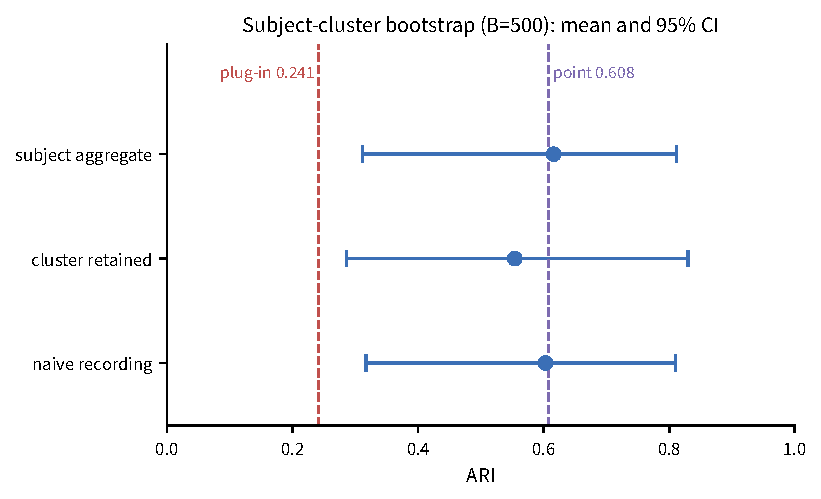
\includegraphics[width=0.85\columnwidth]{fig3_bootstrap_ci.pdf}
\caption{Subject-cluster bootstrap means and percentile intervals for three resampling designs. The intervals sit near the recording point estimate of $0.608$, while the all-subject plug-in of $0.241$ marks the weaker unbalanced regime. They describe resampling spread and carry no coverage guarantee.}
\label{fig:bootstrap}
\end{figure}

A permutation null gives the proper above-chance comparison. The source
labels are permuted relative to the fixed cluster labels, and the
adjusted Rand index is recomputed over two thousand permutations. The
null is centered at zero because the adjusted Rand index is already
corrected for chance, with a ninety-ninth percentile near \(.05\). Every
observed balanced value, from \(.476\) to \(.675\), lies above the
ninety-ninth null percentile.

\begin{table}[H]
\centering
\small
\caption{Permutation null for the balanced adjusted Rand index, with the cluster labels fixed and the source labels permuted. All six observed values exceed the ninety-ninth null percentile. The permutation check supports above-chance association, while the bootstrap intervals remain resampling diagnostics without a coverage theorem.}
\label{tab:permnull}
\begin{tabular}{lcc}
\hline
quantity & permutation null & observed range\\
\hline
mean & .000 & --\\
95th percentile & .030 & --\\
99th percentile & .050 & --\\
adjusted Rand index & -- & .476 to .675\\
\hline
\end{tabular}

\end{table}

\subsection{S5. Secondary analyses and alternative
representations}\label{s5.-secondary-analyses-and-alternative-representations}

\begin{figure}[htbp]
\centering
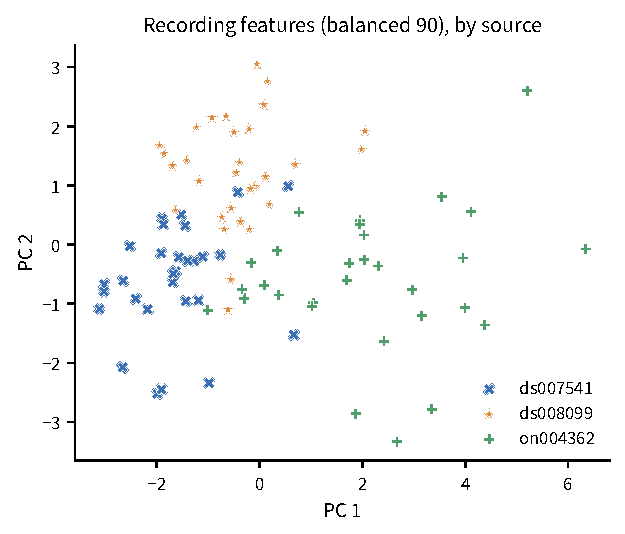
\includegraphics[width=0.85\columnwidth]{fig2_pca_scatter.pdf}
\caption{The balanced ninety recording features projected onto their first two principal components and colored by the true source. One source separates along the first component, while the other two occupy closer but still structured regions; the geometry is consistent with an oracle-$K$ recovery rather than three fully disjoint clouds.}
\label{fig:pca}
\end{figure}

A reference-free bipolar montage lowers the balanced ARI to \(0.415\),
and a surface Laplacian raises it to \(0.678\), both clearly positive.
Dropping any one of the four shared channels leaves ARI between \(0.34\)
and \(0.42\), so no single channel drives the result, though distributed
bad channels or a shared device fingerprint are not excluded. Recovery
persists across representations while its magnitude is
representation-dependent, and strict reference invariance is not
claimed.

\begin{figure}[htbp]
\centering
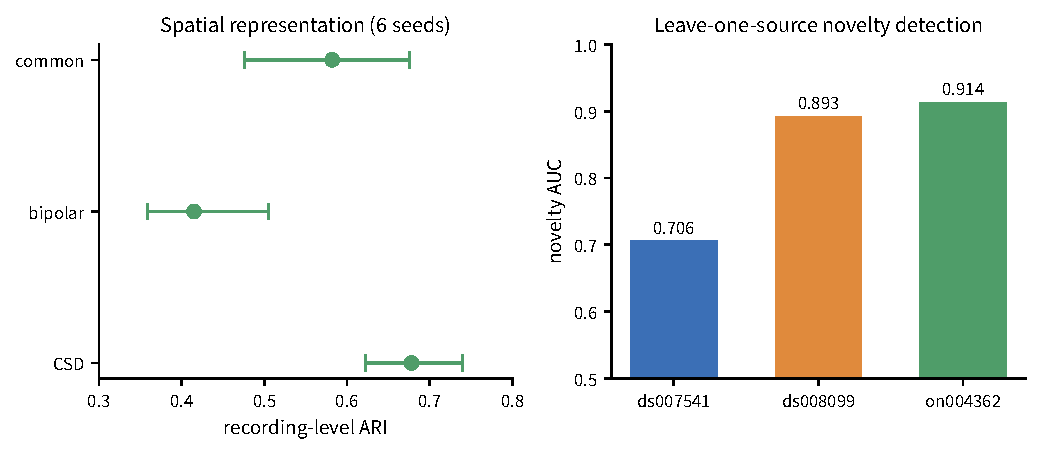
\includegraphics[width=\textwidth]{fig4_spatial_novelty.pdf}
\caption{Left: recording-level ARI under common-average, bipolar, and surface-Laplacian (CSD) spatial representations across six seeds, with the magnitude varying but staying positive. Right: leave-one-source novelty ROC AUC, high for two sources and weak for the third.}
\label{fig:spatial}
\end{figure}

For novelty detection, each source is held out in turn, the scaler and
two centers are fitted on the other two and frozen, and the held-out
recordings are mapped without a refit. Two held-out sources are clearly
detectable as novel, with ROC AUC between \(0.89\) and \(0.93\), while
the third is weakly separated at \(0.70\). Novelty detection is not the
same as correctly labeling a new environment, and full cross-domain
generalization remains unproved.

\subsection{S6. Operational variants}\label{s6.-operational-variants}

The name DELVE covers more than one object, and the guarantee attaches
to exactly one of them. The population alignment that the theorems use
is a compatibility condition, assumed on the population objective rather
than derived from the covariance generative model.

\begin{table}[H]
\centering
\small
\caption{The three operational variants of DELVE and the guarantee attached to each. A fitted StandardScaler is data-dependent even when frozen afterwards, so it is not the pre-given transformation in the theorem and is treated as an empirical variant. Only DELVE-G, with fixed $K$, a pre-given transformation, and a global K-means optimizer, is covered in full by the risk-gap guarantee.}
\label{tab:variants}
\begin{tabular}{lllll}
\hline
Variant & $K$ & scaler & optimizer & guarantee\\
\hline
DELVE-G & fixed & pre-given & global K-means & risk-gap\\
DELVE-L & fixed & pre-given & finite Lloyd & explicit $\delta_{\rm opt}$\\
DELVE-B & blind & data-dependent & Lloyd + selector & none\\
\hline
\end{tabular}

\end{table}

\begin{table}[H]
\centering
\footnotesize
\caption{Blind selector eligibility diagnostics. The parenthesized yes/no marks whether each candidate passes the eligibility gate, stability at or above the adaptive threshold and a positive silhouette. Candidates $K=4,5,6$ never pass the gate in any seed. When both $K=2$ and $K=3$ are eligible, the lower BIC selects $K=3$.}
\label{tab:gatediag}
\begin{tabular}{llllllll}
\hline
seed & K=2 sil & K=2 stab & K=3 sil & K=3 stab & threshold & eligible & chosen\\
\hline
0 & .319 & .899 (yes) & .203 & .724 (no) & .809 & 2 & 2\\
1 & .302 & .893 (yes) & .247 & .849 (yes) & .804 & 2,3 & 3\\
2 & .290 & .803 (yes) & .230 & .831 (yes) & .748 & 2,3 & 3\\
3 & .309 & .907 (yes) & .219 & .824 (yes) & .816 & 2,3 & 3\\
4 & .304 & .840 (yes) & .215 & .624 (no) & .756 & 2 & 2\\
5 & .288 & .795 (yes) & .214 & .691 (no) & .716 & 2 & 2\\
\hline
\end{tabular}

\end{table}

\subsection{S7. Pre-given transformation and three-way
split}\label{s7.-pre-given-transformation-and-three-way-split}

The theorem uses a pre-given, deterministic transformation. Two
empirical checks separate that setting from the data-dependent
StandardScaler. Each uses the balanced ninety recordings, thirty per
source, and the same six seeds as the main table.

\begin{table}[H]
\centering
\footnotesize
\caption{Balanced $K=3$ ARI. The identity transformation is pre-given and gives mean ARI .324 (std .035), above chance but weaker than the fitted StandardScaler at .582 (std .062). The raw feature columns differ in scale, so without scaling K-means is dominated by the large-variance columns. The StandardScaler result is an empirical variant and carries no theorem.}
\label{tab:prefixed}
\begin{tabular}{lllllll}
\hline
transformation & s0 & s1 & s2 & s3 & s4 & s5\\
\hline
pre-given identity ARI & .345 & .365 & .324 & .353 & .290 & .268\\
StandardScaler ARI & .608 & .589 & .476 & .535 & .607 & .675\\
\hline
\end{tabular}

\end{table}

\begin{table}[H]
\centering
\footnotesize
\caption{Strict three-way split. Within each source, ten recordings fit the scaler, ten fit the centers, and ten are held out, so the scaler is independent of the center fit and the evaluation set. Held-out ARI averages .470 (std .101) and NMI averages .528. The center-fit ARI is more variable because it uses only thirty recordings. This is an inductive empirical check, not a conditional theorem.}
\label{tab:threeway}
\begin{tabular}{lllllll}
\hline
quantity & s0 & s1 & s2 & s3 & s4 & s5\\
\hline
center-fit ARI & .802 & .717 & .205 & .578 & .189 & .555\\
held-out eval ARI & .577 & .613 & .343 & .382 & .403 & .500\\
held-out eval NMI & .603 & .640 & .378 & .401 & .518 & .626\\
\hline
\end{tabular}

\end{table}

\subsection{S8. Fixed-window control}\label{s8.-fixed-window-control}

The fixed-window control rebuilds every recording from nine windows, the
smallest common count. Recordings with more windows contribute nine
randomly drawn windows, and the balanced protocol is then run over the
six clustering seeds. The fixed count also fixes the effective duration
at thirty-six seconds.

\begin{table}[H]
\centering
\footnotesize
\caption{Fixed-window versus full-window balanced ARI. The fixed-window row averages the ten window draws within each clustering seed. Full-window mean is .582 (std .068) and fixed-window mean is .577 (std .045). Across the ten window draws and six seeds the sixty fixed-window measurements have a standard deviation of .062. The difference is within the run-to-run spread, so equalizing the window count does not materially change the partition. It removes only the window-count confound, not the other dataset-level factors.}
\label{tab:fixedwindow}
\begin{tabular}{lllllll}
\hline
design & s0 & s1 & s2 & s3 & s4 & s5\\
\hline
full-window ARI & .608 & .589 & .476 & .535 & .607 & .675\\
fixed-window ARI & .589 & .583 & .495 & .563 & .619 & .610\\
\hline
\end{tabular}

\end{table}

\subsection{S9. Expanded balanced Monte Carlo and unbalanced macro
metrics}\label{s9.-expanded-balanced-monte-carlo-and-unbalanced-macro-metrics}

The expanded Monte Carlo repeats the balanced draw independently a
hundred times. Each draw selects thirty recordings per source, fits the
scaler and three-cluster K-means, and scores the result against the
source labels. The six prespecified seeds remain the confirmatory
subset. Precision and recall are computed after Hungarian alignment,
which maps each cluster to the source with which it shares the most
recordings.

\begin{table}[H]
\centering
\footnotesize
\caption{Per-source precision and recall in the balanced Monte Carlo, with macro averages in the overall column, and unbalanced macro precision and recall alongside. The balanced macro F1 is .850 and the unbalanced macro F1 is .710. Balanced ARI is .606 (std .100) and unbalanced ARI is .371. The Monte Carlo spread is a sampling distribution, not a confidence interval with a coverage theorem.}
\label{tab:montecarlo-supp}
\begin{tabular}{lcccccc}
\hline
quantity & source 1 & source 2 & source 3 & overall & unbalanced & --\\
\hline
per-source precision & .863 & .826 & .901 & .863 & .731 & --\\
per-source recall & .838 & .936 & .777 & .850 & .786 & --\\
\hline
\end{tabular}

\end{table}

\subsection{S10. Gate-parameter and candidate-range
sensitivity}\label{s10.-gate-parameter-and-candidate-range-sensitivity}

The gated selector contains several fixed constants, so the gate is
recomputed over a grid of stability caps, multipliers, silhouette-gate
settings, and candidate ranges. The clustering and the per-\(K\) metrics
are held fixed; only the decision rule changes. The silhouette gate on
or off gives the same result at every setting, because the candidates
that reach the stability threshold all have positive silhouette, so only
the silhouette-on rows are shown.

\begin{table}[H]
\centering
\footnotesize
\caption{Number of seeds selecting $K=3$ across nine cap and multiplier combinations. The entries are the same with the silhouette gate disabled. Across all eighteen variants, including the on/off gate, the mean $K=3$ frequency is 2.56 out of six. The lower multiplier over-splits to four clusters and the higher multiplier merges to two, so no setting raises the recovery rate beyond three seeds.}
\label{tab:gatesens}
\begin{tabular}{lccc}
\hline
cap \textbackslash{} mult & .8 & .9 & 1.0\\
\hline
.80 & 3/6 & 3/6 & 3/6\\
.85 & 3/6 & 3/6 & 1/6\\
.90 & 3/6 & 3/6 & 1/6\\
\hline
\end{tabular}

\end{table}

\begin{table}[H]
\centering
\footnotesize
\caption{Candidate-range sensitivity at the prespecified cap .85 and multiplier .9. Widening the range does not change the choice, because the decision is settled between two and three clusters before the higher candidates enter. The full baseline comparison is in the main-text selector table.}
\label{tab:rangesens}
\begin{tabular}{lcc}
\hline
candidate range & selected $K$ (s0–s5) & $K=3$ count\\
\hline
2–4 & 2,3,3,3,2,2 & 3/6\\
2–5 & 2,3,3,3,2,2 & 3/6\\
2–6 & 2,3,3,3,2,2 & 3/6\\
\hline
\end{tabular}

\end{table}
